%% Please fill in your name and collaboration statement here.
\newcommand{\studentName}{**FILL IN YOUR NAME HERE**}
\newcommand{\collaborationStatement}{**FILL IN YOUR COLLABORATION STATEMENT HERE \\ (See the syllabus for information)**}


%%%%%%%%%%%%%%%%%%%%%%%%%%%%%%%%%%%%%%%%%%%%%%%
\documentclass[solution, letterpaper]{cs121}
\usepackage{enumerate}
\begin{document}
\header{1}{Tuesday September 22, 2015 at 11:59pm}
\textit{Note: Finite automata (FA) drawings may be done by hand or using an online drawing tool.}
%%%%%%%%%%%%%%%%%%%%%%%%%%%%%%%%%%%%%%%%%%%%%%%
\PART{Sam and Serena}
%%%%%%%%%%%%%%%%%%%%%%%%%%%%%%%%%%%%%%%%%%%%%%%
\problem{2+2+1}{3 lines}

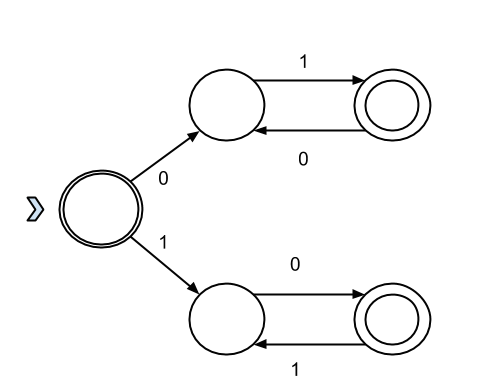
\includegraphics[width=7.0cm]{1-2a.png} 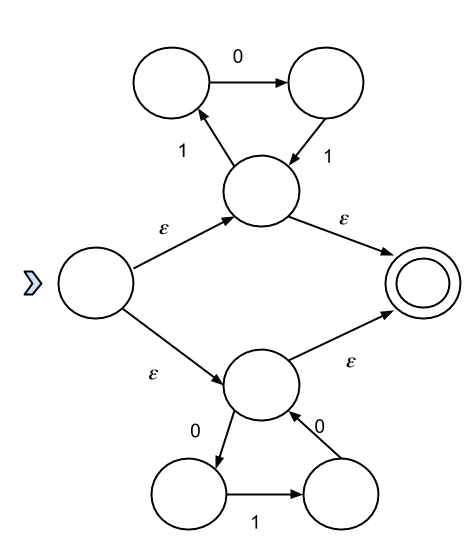
\includegraphics[width=7.0cm]{1-2b.png}\\\\
\subproblem Describe informally $L_1$, the language accepted by the NFA on the left.\\
\subproblem Describe informally $L_2$, the language accepted by the NFA on the right.\\
\subproblem Write down $L_1 \cap L_2$.
\\\\
\noindent {\bf Solution.}

\pagebreak

\problem{3+6+(2)}{1 page}
Let $S_n = \{1, 2, 3, ..., n\}$. We can represent subsets of $S_n$ using strings of length $n$ by setting the $i^{th}$ character to 1 if element $i$ is in the subset, and 0 if it is not. For example, for $n = 3$, the subset $\{3\}$ would be represented by the string $001$, and the subset $\{2, 3\}$ would be represented by the string $011$. Let $f_n : \{0, 1\}^n \to P(S_n) $ be a function that produces the subset represented by a string, e.g. $f_3(001) = \{3\}$ and $f_3(011) = \{2, 3\}$.

\subproblem Is $f_n$ injective for all $n$? Surjective? Bijective? Informally explain each of your answers.

\subproblem In this question, we will use the machinery of DFAs to ``compute'' a function. We will label accept states with values, and the state that the DFA halts at after processing an input string will correspond to the output of the function it computes. Your task is to draw a DFA that computes the function $f_3$. \textit{Notes: } 
\begin{itemize}
\item If the DFA is given a string of length greater than 3, it should enter a labeled ``error'' non-accept state. 
\item If the DFA is given a string of length 3, it should halt in an accept state that corresponds to the correct subset of $S_3$.  Thus you should have $2^3 = 8$ accept states. 
\item No additional explanation or description of the DFA is required beyond the drawing. 
\item Label the accept states in your drawing. An example of a labelled accept state that should appear in your drawing is below:\\
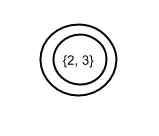
\includegraphics[width=3cm]{1-1ex.png}
\end{itemize}
\subproblem (Challenge!! Not required; worth up to 2 extra credit points.) How many states are required for a DFA that computes $f_n$? Prove that your answer is a lower bound.\\\\
\textit{Note: On every problem set we will provide a challenge problem, generally significantly more difficult than the other problems in the set, but worth only a few points. It is recommended that you attempt these problems, but only after completing the rest of the assignment.} 
\\\\
\noindent {\bf Solution.}
\pagebreak
%%%%%%%%%%%%%%%%%%%%%%%%%%%%%%%%%%%%%%%%%%%%%%%
\PART{Juan and Varun}
%%%%%%%%%%%%%%%%%%%%%%%%%%%%%%%%%%%%%%%%%%%%%%%
\problem{5+5}{1/2 page}

Two FAs are ``equivalent'' if the languages that they accept are the same. If two FAs are not equivalent, they are ``distinct''. For this question, you may assume that the alphabet is $\{0, 1\}$.

\subproblem How many distinct DFAs are there with 1 state? Draw it/them. Describe informally the languages recognized by each.

\subproblem How many distinct NFAs are there with 1 state? Draw it/them. Describe informally the languages recognized by each.
\\\\
\noindent {\bf Solution.}

\problem{3+3+3}{1/3 page}
Are the following statements true or false? Justify your answers with a proof or counterexample.\\
\subproblem $(L_1 \cap L_2)^* = L_1^* \cap L_2^*$

\subproblem $(L_1 \cup L_2) \cdot L_3 = (L_1 \cdot L_3) \cup (L_2 \cdot L_3)$, where $\cdot$ is concatenation.

\subproblem $\{ \vareps\} \cdot L_1 = \emptyset \cdot L_1$
\\\\
\noindent {\bf Solution.}

\end{document}